
%%%%%%%%%%%%%%%%%%%%%%% file typeinst.tex %%%%%%%%%%%%%%%%%%%%%%%%%
%
% This is the LaTeX source for the instructions to authors using
% the LaTeX document class 'llncs.cls' for contributions to
% the Lecture Notes in Computer Sciences series.
% http://www.springer.com/lncs       Springer Heidelberg 2006/05/04
%
% It may be used as a template for your own input - copy it
% to a new file with a new name and use it as the basis
% for your article.
%
% NB: the document class 'llncs' has its own and detailed documentation, see
% ftp://ftp.springer.de/data/pubftp/pub/tex/latex/llncs/latex2e/llncsdoc.pdf
%
%%%%%%%%%%%%%%%%%%%%%%%%%%%%%%%%%%%%%%%%%%%%%%%%%%%%%%%%%%%%%%%%%%%


\documentclass[runningheads,a4paper]{llncs}

\usepackage{amssymb}
\usepackage{listings}

\lstdefinelanguage{json}
{
    morestring=[b]",
    morestring=[d]'
}

\setcounter{tocdepth}{3}
\usepackage{graphicx}

\usepackage{url}
\urldef{\mails}\path|{smsohan, frank.maurer}@ucalgary.ca|
\newcommand{\keywords}[1]{\par\addvspace\baselineskip
\noindent\keywordname\enspace\ignorespaces#1}

\begin{document}

\mainmatter  % start of an individual contribution

% first the title is needed
\title{Practical Challenges with Web Service Evolution:\\A Review of Literature and Current Industry Practices}

% a short form should be given in case it is too long for the running head
\titlerunning{Challenges with Web Service Evolution}

% the name(s) of the author(s) follow(s) next
%
% NB: Chinese authors should write their first names(s) in front of
% their surnames. This ensures that the names appear correctly in
% the running heads and the author index.
%
\author{S M Sohan%
\and Frank Maurer}
%
\authorrunning{Challenges with Web Service Evolution}
% (feature abused for this document to repeat the title also on left hand pages)

% the affiliations are given next; don't give your e-mail address
% unless you accept that it will be published
\institute{University of Calgary\\
\mails\\
\url{http://ucalgary.ca}}

%
% NB: a more complex sample for affiliations and the mapping to the
% corresponding authors can be found in the file "llncs.dem"
% (search for the string "\mainmatter" where a contribution starts).
% "llncs.dem" accompanies the document class "llncs.cls".
%

\toctitle{Lecture Notes in Computer Science}
\tocauthor{Authors' Instructions}
\maketitle


\begin{abstract}


Service-oriented Systems often rely on integrating software systems that are developed by independent parties and that evolve independently. In this paper we identify the key challenges with web service evolution such as backward and forward compatibility, serving and testing multiple concurrent versions, version specific documentation, communicating future changes. Following an appropriate strategy to overcome these challenges will enable web service publishers to iterate their services as required while minimizing the impact on existing consumers of the services. To understand and deal with these challenges, we performed a systematic review of the existing literature on web service evolution and investigated three real world web services. Based on our findings, we discussed the challenges and opportunities for future work to address the challenges.

\keywords{Web Service, Evolution, Versioning, SOA, SOAP, REST}
\end{abstract}


\section{Introduction}

Web services offer a web-based communication mechanism between two software systems, commonly known as web service publishers and consumers. W3C defines web services as follows \cite{w3c_web_service}:

\begin{quote}
``A Web Service is a software application identified by a URI [IETF RFC 2396], whose interfaces and binding are capable of being defined, described and discovered by XML artifacts and supports direct interactions with other software applications using XML based messages via Internet-based protocols.''
\end{quote}

However, in todays technology multiple messaging formats in addition to XML are used. Wikipedia provides a generic definition of web services as follows: \cite{web_service_wiki}:

\begin{quote}
``A web service is a method of communication between two electronic devices over the World Wide Web. A web service is a software function provided at a network address over the web or the cloud, it is a service that is ``always on'' as in the concept of utility computing.''
\end{quote}

For example, a geographical mapping web service may be consumed by many different kinds of consumers in real life such as: real-estate listing web sites, local business search portals, transit information web sites, etc. Similarly, payment processing web services are used by a multitude of consumers such as: e-commerce applications, retail stations etc.

To carry out the actual communication, the web service publishers and consumers follow specific protocols. Of the many protocols that are in use today \cite{web_service_protocols_wiki}, two commonly used protocols are as follows:

\begin{itemize}
  \item Simple Object Access Protocol or \textbf{SOAP} web services
  \item Representational State Transfer or \textbf{RESTful} web services
\end{itemize}

Due to their historical usage, the term ``web service'' is often interpreted as SOAP. However, throughout this paper, unless otherwise specified, we have used this term to represent a web based communication method between two software systems irrespective of their actual implementation details. The findings mentioned in this paper are based on SOAP and REST based services due to their relative popularity over the other types.

\subsection{SOAP Web Services} % (fold)
\label{sub:soap_web_services}
SOAP was designed in 1998 by Winer et al. for Microsoft and is currently maintained by the World Wide Web Consortium \cite{soap_wiki}. In brief, SOAP is an XML based protocol to communicate structured data and necessary headers between the consumers and publisher of a web service.

A SOAP web service is composed of one or more operations or methods. SOAP XML messages are used for communication between a consumer of the web service and its methods. The structure of these methods, their corresponding messages and other meta information of a SOAP service can be described using an accompanying XML based Web Services Description Language or WSDL file. In addition to providing a structured definition of the service, these WSDL files can be automatically parsed by code-generators to provide the consumers with an easy to integrate interface.

% subsection soap_web_services (end)

\subsection{RESTful Web Services} % (fold)
\label{sub:restful_web_services}
Being an XML based protocol, SOAP messages are often verbose. Also, the additional header information introduces communication overheads. On the other hand, RESTful web services gained popularity with the rise of cloud computing as they provide a lightweight and flexible approach \cite{mangler2010origin}, where the HTTP protocol stack is leveraged without imposing constraints on the actual format of the messaging.

The term Representational State Transfer (REST) was introduced by Roy Fielding \cite{rest_wiki} and is used interchangeably as RESTful web service or Web API. In brief, REST is an implementation for web services where user defined ``resources'' are created, accessed, modified and deleted utilizing the various features of the HTTP stack such as caching, security, layering and different request methods (GET, POST, PUT, DELETE etc.), content types.

% subsection restful_web_services (end)

The scope of this paper is limited to only the evolutionary aspects of web services. On this topic, the remainder of this paper is organized as follows: in the next section we discuss the motivation behind this research followed by our research questions. Then, we discuss the research method and findings in Sections \ref{sec:research_method} and \ref{sec:research_findings} respectively. Finally, we present the key challenges and future work opportunities with evolving web services in Section \ref{sec:discussion}.

\section{Motivation} % (fold)
\label{sec:motivation}
Web services, like other software systems, need to evolve to stay on top of bugs and ever changing requirements. For example, between May 15th 2013 and May 22nd 2013, the Facebook API team saw 238 new bugs, resolved 211 bugs and fixed 24 bugs \cite{facebook_release_note}. However, often times web services are used by an unknown number of consumers, and the web service publishers have little control over them. Updating a web service can be tricky in such a situation since a breaking change may upset the existing consumers. To be able to evolve in such a decoupled scenario, multiple versions of a service need to coexist which poses both technical and business challenges in multiple fronts. At a conceptual level, Figure \ref{fig:web_service_layers} shows the different parts of a web service that need to deal with evolution challenges:


\begin{figure*}[ht]
  \centering
  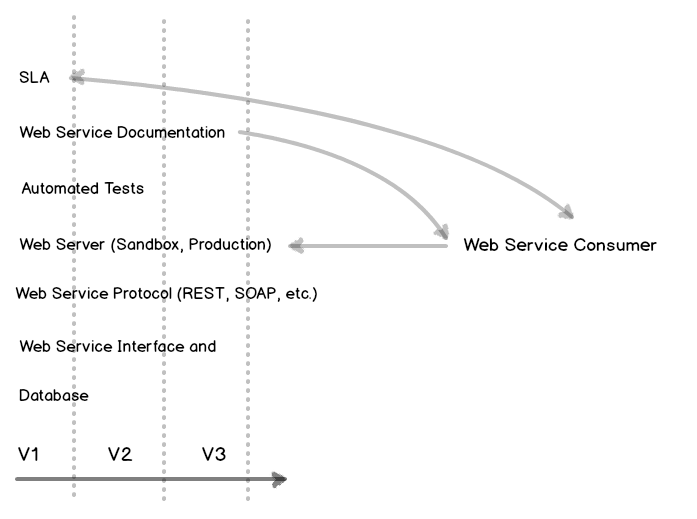
\includegraphics[width=\textwidth]{web_service_layers.png}
    \caption{Different Parts of an Evolving Web Service}
  \label{fig:web_service_layers}
\end{figure*}

As shown in Figure \ref{fig:web_service_layers}, the different parts of a web service need to cope with the changing requirements for its evolution. However, there is a little to no standard approach to tackle these parts of an evolving web service. The motivation for this research stems from the need to improve this situation.

% section motivation (end)

\section{Research Questions} % (fold)
\label{sec:research_questions}
To better understand the challenges related to web service evolution we have focused on the following list of research questions:

\begin{itemize}
  \item Why do web services need to evolve?
  \item How to evolve the web services?
  \item What are the key challenges for evolving web services?
\end{itemize}

Focusing on these questions helped us identify some of the gaps of the currently available techniques for evolving web services. Using this as a background, innovative future work can be carried out to fill these gaps and simplify web service evolution.
% section research_questions (end)

\section{Research Method} % (fold)
\label{sec:research_method}

We have performed a Systematic Literature Review to extract information from the published articles following \cite{kitchenham2007guidelines}. We have also investigated three published real-word web services to find out the answers to the research questions based on todays solutions.
In this regard, we have limited our research to two high level sources as follows:

\begin{itemize}
  \item Published articles from the academia and the industry
  \item Real world web services
\end{itemize}

\subsection{Systematic Literature Review} % (fold)
\label{sub:systematic_literature_review}
Kitchenham et al. defines systematic review as follows \cite{kitchenham2007guidelines}:

\begin{quote}
``A form of secondary study that uses a well-defined methodology to identify, analyse and interpret all available evidence related to a specific research question in a way that is unbiased and (to a degree) repeatable.''
\end{quote}
We have carried out a systematic review because it helped us examining and summarizing the relevant work from the existing literature. To this regard, we have identified relevant papers from the following sources: IEEExplore, ACM Digital library, Google Scholar, Citeseer library, ScienceDirect, and SpringerLink.

To identify the relevant papers from these sources we have performed keyword searches. As mentioned in \cite{petersen2008systematic}, keywording is a two step process, 1) extracting keywords from reading the abstracts and, 2) combining keywords from different papers. At step 1, we initially searched for the papers containing the terms ``web service''. We have seen repeated mentions of the terms Service Oriented Architecture or SOA, SOAP, Web API and REST to denote similar concepts in these papers. In addition to this, we have expanded the word ``evolution'' with its commonly used English synonyms. At step 2, we combined the keywords and formed the following pseudo search query:

\textbf{(``Web Service'' OR SOA OR SOAP OR RESTful OR ``Web API'')  AND (evolve OR evolution OR versioning)}

We searched the aforementioned sources using this query in the title, abstract and keywords of the published articles. However, the sources offer different search capabilities and attempts were made to tune the queries based on the capabilities of a source. For example, only article titles were searched on Google Scholar and SpringerLink as they don't allow search in abstracts at the time of writing this paper. We found the following number of matches from the sources including duplicates:

\begin{tabular}{l c r}
  Source & Fields Searched & Number of Matches \\
  \hline
  IEEExplore & Title, Abstract & 224 \\
  Google Scholar & Title & 130 \\
  ACM Digital Library & Title, Abstract & 235 \\
  ScienceDirect & Title, Abstract, Keywords & 54 \\
  SpringerLink & Title & 15
\end{tabular}

From the search results, we performed a primary screening and selected 21 papers after reading the abstracts. Then, for the remaining articles, we read the full paper as long as it was found relevant, i.e. only if it contained topics about the evolution of web services. The resulting list is composed of \cite{kitchenham2007guidelines} \cite{petersen2008systematic} \cite{treiber2009analyzing} \cite{borovskiy2008evolution} \cite{lublinsky2007versioning} \cite{laskey2008considerations} \cite{wilde2004semantically} \cite{fang2007version} \cite{leitner2008end} \cite{mangler2010origin} \cite{kaminski2006design} \cite{le2008synchronizing} \cite{aversano2005visualizing}.

In the next section, we list and discuss our findings from these selected papers in light of the research questions.

\subsection{Analysis of Real World Web Service Evolution} % (fold)
\label{sub:analysis_of_real_world_web_service_evolution}
In addition to looking at the published articles, we have also analyzed real world web services to examine their approaches to deal with evolution. A comprehensive review of all the real world web services is beyond the scope of this research. However, we selected the following web services as they are evolving with a large number of existing consumers using different evolution approaches:

\begin{itemize}
  \item Google Maps
  \item Twitter API
  \item Facebook Graph API
\end{itemize}

The triangulation of the findings from the systematic literature review and the analysis of real world services provide a broader insight than each method itself.

% subsection analysis_of_real_world_web_service_evolution (end)

% section research_method (end)

\section{Research Findings} % (fold)
\label{sec:research_findings}

\subsection{Systematic Literature Review} % (fold)
\label{sub:literature_review}

\subsubsection{Why Do Web Services Evolve?} % (fold)
\label{sub:why_do_web_services_change}
In this section, we have listed the drivers behind web service evolution as discussed in 3 of the selected papers. To begin with, in \cite{treiber2009analyzing} Treiber et al. provided a list of changes related to web services with their interdependencies. To identify the source and impact of a change, they categorized the stakeholders into four roles:

\begin{itemize}
  \item \textbf{web service provider}, who is responsible for planning and conception of the service
  \item \textbf{developer}, who implements the planned service
  \item \textbf{service integrator}, who integrates with external web services and
  \item \textbf{user}, who actually uses the integrated application.
\end{itemize}

One or more of these roles may be played by one individual. The stakeholders take part in driving changes to a web service. The authors identified the following types of changes in a web services: Interface, Implementation, Quality of Service (QoS), Usage, Requirement, Service-level Agreement (SLA), Pre and post conditions, and Feedback. In line with \cite{treiber2009analyzing}  Lublinsky also pointed out that a new version may be required primarily because of changes in its interface, schema of the message payload or in it’s implementation. In \cite{laskey2008considerations}, Laskey identified the key reasons for changes between versions as: a) service description changes, b) changes in functions, c) changes in the interaction mechanics, and d) change of known pre and post conditions. These changes would require new versions of the service as well as accompanying any explanation of the specific changes.

In addition to the types of changes discussed above, Borovskiy et al. identified some drivers behind web service evolution from the perspective of an enterprise, where both the web service consumer and publisher may be part of the same organization \cite{borovskiy2008evolution}. In this regard, they categorized two classes of drivers behind the evolution of web services as follows:

\begin{itemize}
  \item \textbf{Intrinsic change drivers}: Poor design, Poor implementation quality
  \item \textbf{Extrinsic change drivers}: Market drivers, Differentiation drivers, Business requirement drivers, Operational process drivers, Legislative regulatory drivers, User related drives
\end{itemize}


A change in a web service impacts one or more of the stakeholder roles based on its type. Treiber et al. pointed out that, in addition to stakeholder impacts, the sources are also interdependent on each other \cite{treiber2009analyzing}. For example, when a web service \textbf{provider} decides to change the \textbf{interface}, the \textbf{developer} needs to write the changed interface and its \textbf{implementation}. If the changed interface if not backward compatible, and the service \textbf{integrator} needs to modify the integration. The new interface and implementation may instigate a change its \textbf{QoS}, since it may improve or degrade the performance. The changes may improve or degrade the \textbf{QoS} and impact the \textbf{end user}.

% subsubsection why_do_web_services_change (end)


\subsubsection{How to evolve the web services?} % (fold)
\label{sub:how_to_evolve_the_web_services_}
Now that we have listed the drivers behind web service evolution, next we present the different approaches to tackle web service evolution based on 6 of the selected papers.

\subsubsection{Versioning:} % (fold)
Lublinsky compared between multiple approaches of implementing evolving web services based on different dimensions as follows \cite{lublinsky2007versioning}.

\begin{itemize}

  \item \textbf{Units of versioning}: One approach to version a service is to apply a single version to all it’s methods that can be deployed as a group. Another approach is to version individual methods or operations of the service as they change, this confines the change to only specific methods and provides a finer grained versioning. However, deployment of such versioned methods are complicated and it forces the consumer to specify the service, its method name and an additional version to use for each operation.
  \item \textbf{Service version life-cycle considerations}: Based on the actual need, Lublinsky suggests adjusting the life-cycle of versions, as too many versions increase the maintenance overhead while too few versions leave the consumers a smaller time window to upgrade since each version has a shorter life-cycle.
  \item \textbf{Version deployment/access approaches}: When deploying versioned services, Lublinsky compares between multiple versions deployed on the same endpoint vs. each version deployed on its own endpoint. Lublinsky points out that the former approach may introduce conflicts in names of the objects, databases and other related resources, and requires intermediate routers, which typically lowers performance and may introduce SLA complications. The author favored the latter approach and argued that it provides better scalability and loose coupling between versions.

\end{itemize}

To summarize, this paper paper points out some key trade-offs that need to be addressed while evolving web services based on the specific use case.

A versioning scheme is required to identify and use a specific version. Laskey discusses about the versioning of web services in \cite{laskey2008considerations}. In this paper, the author discussed versions in terms of identifiable resources, that can have multiple versions and are modified by applying new versions to the original one.

To identify a specific version of a resource, Leskey suggests using a unique identifier with an accompanying explanation of how to interpret it. The versioning identifiers should be used consistently. In addition to this, the author also recommends specifying a policy describing compatibility between the versions so the consumers clearly understand the impacts of version changes. As an example, the author mentioned a generic policy as follows:

\begin{quote}
``A versioning scheme for a service may include a generic policy, such as any succeeding version identified as 1.j will be backward compatible with any 1.i previous version in the sense that results are identically generated in version 1.j for functionality that existed in previous 1.i versions.''
\end{quote}

To locate each version, the author provided the following example URL based scheme: \emph{http:///a.b.c/services1/20080601/} , where service1 is the name of the resource and \emph{20080601} is the date based version identifier. Given this URL scheme, the author suggests the service descriptions to dereference the URL and provide necessary details about the version so that the versioning information is transparent to the consumers.

\subsubsection{Implementation:}
Once an appropriate evolution and versioning strategy is selected, the required changes need to be implemented. Next, we discuss the implementation approaches as suggested in the literature from the perspective of two levels, \textbf{1) protocol level} and \textbf{2) application level.}

\subsubsection{Protocol Level Implementation:}
Since web services typically follow a protocols such as SOAP, REST, etc., protocol level support for evolving web services would allow for uniform standards. In \cite{wilde2004semantically} Wilde proposed a conceptual framework for SOAP web services where consumers can be forward compatible in a managed way.

At it’s core, the framework includes open and extensible XML schemas so the consumers of old version can work with the schema in a newer version. In addition to this, the framework recommends using a set of custom extensions to the XML schema. These extensions can be as simple as XML tags such as mustUnderstand, mayIgnore or some complex ones to suit the specific use case in hand. But irrespective of their actual usage, an accompanying guideline on their processing rules need to be provided. Using the approach of this framework, the consumers of the web service can attain a predictable level of ``graceful degradation'' as the service evolves.

Using a similar approach but instead of arbitrary custom tags to extend the schema, Fang et al. provides a concrete list of six XML nodes to create a version-aware service model for SOAP web services \cite{fang2007version}. They introduced extensions to WSDL and UDDI to tackle evolving web services. These extensions are composed of six XML nodes: \textbf{1) version name, 2 ) version description, 3) startTime of the version, 4) endTime of the version, 5) alias such as (new, current etc) of the version name and, 6) original version that preceded it}.

With the help of this versioning description of the service, a consumer can find and register for a target version through a service registry. The server can publish events as new a version of a service is deployed and the registered consumers can subscribe to these events. When a new version is released, the consumer gets notified about the change and can self update if the changes are backward compatible. The authors discussed an example implementation of this approach and demonstrated that using this approach SOAP services can be versioned and future changes can be communicated to the consumers.

In \cite{leitner2008end} Leitner et al. provided an alternative approach to transparently handle multiple versions of SOAP web services using their framework called VRESCo. At it’s core, VRESCo builds a graph of the versions showing predecessor relations as shown in Figure \ref{fig:vresco}:

\begin{figure*}[ht]
  \centering
  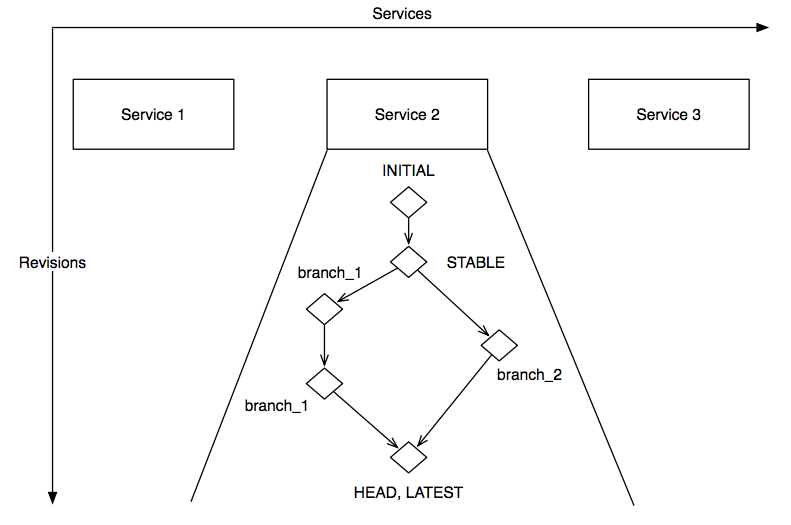
\includegraphics[width=\textwidth]{vresco.png}
    \caption{VRESCo Service Version Graph, source: \cite{leitner2008end}}
  \label{fig:vresco}
\end{figure*}


For each version, VRESCo uses a free-form tag to identify it. The version tag and associated meta information from the WSDL file of each version is stored in VRESCo's database. So, when new versions are released, it can perform an analysis to see if the changes are backward compatible. To route a consumer request to the right version, the versions of a service are deployed behind a proxy. Based on a ``selection strategy'' specified by the consumer (e.g. always use latest, always use stable, fix version, etc.) the proxy can then automatically select the desired version without needing the consumer to change it’s implementation. For compatible updates, this approach off-loads the consumer at the expense of an additional proxy layer.

In addition to the protocol level evolution support for SOAP web services, Mangler et al. showed a solution for RESTful web services in \cite{mangler2010origin}. They introduced a description language called RIDDL for RESTful web services to support service composition and evolution.

RIDDL adds XML based descriptions to RESTful web services. Using RIDDL, service evolution is expressed through a chain of adapters, where the output of a service matches with the input of its preceding version. From this XML declaration of the chain, it is possible to merge the inputs and outputs from each adapter to create a full description of a specific version.

\subsubsection{Application Level Implementation:}

Following from the protocol level implementation approaches discussed in the previous section, we have presented the application code level solution approaches in this section.

Kaminski et al. presented a design technique for evolving web services from the perspective of the source code implementation \cite{kaminski2006design}. They identified some key requirements for their design such as: \textbf{a) backward compatibility, b) common data store, c) no code duplication, d) untangled versions, e) unconstrained evolution, and f) a visible mechanism}.

With these requirements laid out, they proposed a design technique called ``Chain of Adapters'' for the implementation of evolving web services. Figure \ref{fig:chain_of_adapters} shows a high level view of the design.

\begin{figure*}[ht]
  \centering
  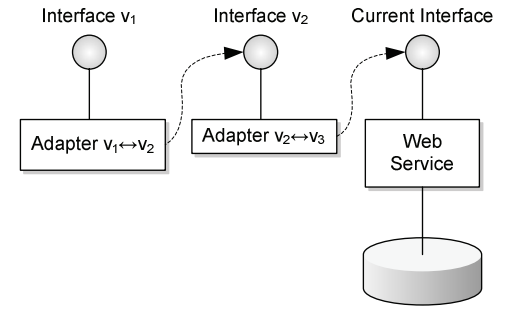
\includegraphics[width=\textwidth]{chain_of_adapters.png}
    \caption{Chain of Adapters structure, source: \cite{kaminski2006design}}
  \label{fig:chain_of_adapters}
\end{figure*}

In essence, the design technique can be described as follows: To start with, a web service can be developed as usual. Then, the interface of the web service is duplicated under a namespace V1. An implementation of this interface is created in the same V1 namespace that performs necessary translations on the data and delegates the methods to the original web service. This produces a snapshot of the V1 service which can be published for its consumers.

Now, to evolve to V2 of the service, the changes are made to the original web service. A compensating in a V1 $\leftrightarrow$ V2 adapter is created to translate the V1 service to the changed web service. This V1 $\leftrightarrow$ V2 adapter is the first of the ``Chain of Adapters'' to be used for evolution. Once the changes are complete, the interface of the original web service is duplicated into a the V2 namespace. In the same namespace, an implementation of this V2 interface delegates the calls to the original web service, while the V1 $\leftrightarrow$ V2 adapter targets this new implementation. This way, a new snapshot for the V2 of the service is created.

As the service evolves, introducing new adapters for each version would produce a chain of such adapters to ensure backward compatibility and code reuse while being able to serve multiple concurrent versions.

The ``Chain of Adapters'' technique addresses their requirements, but they mentioned some caveats. For example, the adapters need to ensure all breaking changes are compensated, which my need for a separate data store when fields are removed from the datastore on subsequent versions. Also, this chain effectively connects all the versions, so a bug or it’s fix on one version may have impact on all the versions.

\subsubsection{Communication:}
A change in a web service may impact multiple stakeholders. So, it is important to communicate the changes and their impacts to the stakeholders as the service evolves. In this section, we have discussed 2 of the selected papers as they suggested ways to effectively communicate the evolution of web services.

In \cite{le2008synchronizing} Zou et al. presents a technique to generate consumer specific changelogs for evolving SOAP web services. For existing consumers, the authors presented an approach where a consumer specific changelog can be generated based on their usage pattern of the service. The approach is described below:

\begin{itemize}
  \item \textbf{Service invocation monitoring}: a monitoring system is used to track the usage pattern of each consumer so when a service is changed, it can identify specific areas of interest for a consumer
  \item \textbf{Service difference analysis}: Since SOAP services are described using XML based WSDL files, the differences between the two versions such as addition, removal or modification can be analyzed by comparing the WSDL files
  \item \textbf{Release note customization}: The release note can then be tailored for each consumer by using the data collected at step 1 to only include relevant changes per customer
  \item \textbf{Code release note linkage}: Using the customized release note from step 3, it is possible automatically inspect the consumer code and discover fragments of the code that need to change for the new version.
\end{itemize}

Aversano et al. provided an alternate approach to communicate changes in SOAP web services using a graphical way in \cite{aversano2005visualizing}. To construct the graphical representation, the authors extracted meta information about methods and parameters for SOAP web services from the WSDL files. This meta information is then presented in a graph to visualize the service with its methods and parameters, and highlight changes between versions.

% subsubsection how_to_evolve_the_web_services_ (end)

% subsection literature_review (end)

\subsection{Analysis of Real World Web Service Evolution} % (fold)
\label{sub:review_of_industry_examples}

In this section we have listed our findings from the following real world evolving web services:

\begin{itemize}
  \item \textbf{Google Maps}: Google Maps provides a web service for its consumers and updates the service to provide ``new features, bug fixes and performance improvements'' \cite{google_maps_versioning}.
  \item \textbf{Twitter Web API}: Twitter provides a RESTful web service to interact with its data from third-party applications \cite{twitter_api}. This web service is also evolving to fix bugs and bring new features, but using a different approach from that of Google Maps.
  \item \textbf{Facebook Graph API}: Facebook Graph API is the primary web service to retrieve and post data to Facebook \cite{facebook_api}. The service evolves to support change/removal of functionality, backwards compatibility, Facebook product changes, and privacy and security related changes.
\end{itemize}

\subsubsection{Versioning:} % (fold)
\label{sub:versioning}
Google Maps uses the following versioning policy \cite{google_maps_versioning}:

\begin{itemize}
  \item \textbf{Experimental version}: With all the latest features, bug fixes and improvements. But this version is not guaranteed to be feature stable.
  \item \textbf{Release version}: From the the experimental version, every quarter, a feature stable version of the service is tagged as a ``release'' version. These release versions may receive bug fixes but the features remain stable.
  \item \textbf{Previously released or Frozen version}: Every time a new ``release version'' is tagged, the oldest existing release version is ``frozen'', so no new features or bug fixes are applied to ensure it remains completely feature stable.
\end{itemize}
Every time a new release version is tagged, the oldest version is retired. Google Maps guarantees the versions are backward compatible and automatically migrates the consumers using the oldest version to the following version without needing the consumers to make any change on their ends.

On the other hand, the Twitter API had two versions at the time of writing this paper \cite{twitter_api} and the old version is marked as deprecated. The users of the old version are suggested to upgrade to the new version before its posted date of expiry. Once a version is released, future changes are made to the released version to provide new features and bug fixes. However, unlike Google Maps, new features are not always released under a new version name. Instead, the changes may be deployed under the same version name.

Unlike the previous approaches, Facebook Graph API on the other hand uses a different approach for its evolution. They have a 90-day breaking change policy stated as follows: \cite{facebook_api}

\begin{quote}
``Platform changes that would require a code change from developers (security and privacy changes excluded) will be announced at least 90 days before the change goes into effect.''
\end{quote}

The service consumers, aka platform developers, can opt-in to migrate to a new release to get an early look on the impact of the breaking changes specific to their use case and take necessary actions within the 90-day period. All users are automatically migrated to the new version after this 90-day period.

Both Google Maps and Twitter web service users identify a desired version of the service in the URL. For example, to use the version 3.12 of Google Maps API, the following URL can be used https://maps.googleapis.com/maps/api/js?v=3.12. In absence of a version parameter, by default the experimental version of Google Maps is used.

Instead of a URL based versioning identifier, Facebook allows the consumers to enable the changes by pushing a button on the Facebook website. Once enabled, the users can make necessary changes before the 90-day period.

\subsubsection{Documentation:}
Google Maps web service provides a human readable documentation of the service operations with example requests and responses specific to a version \cite{google_maps_services}. Since the API is publicly available, the users can run the example requests to produce live results by browsing the API endpoints on their browsers.

Twitter also publishes human readable API documentation for each version of the web service in their developer portal \cite{twitter_api}. The portal also includes an interactive web browser based console to let its users explore the service on the browser \cite{twitter_console}.

Similarly, the Facebook Graph API accompanies both a static HTML based and an interactive the API called ``Graph API Explorer'' \cite{facebook_api}.

\subsubsection{Communication:}

The real-world web services use multiple channels to communicate with the users. For example, Google Maps web service uses StackOverflow.com to collect code related questions from the users, an issue tracker to let the users report defects, and blogs and an email group to discuss changes \cite{google_maps_forum}.

To communicate the past and upcoming web service changes, Twitter publishes a ``Calendar of API Changes'' on their developer portal \cite{twitter_calendar}. In addition to this calendar, the portal also has developer blogs, a discussion forum and an issue tracker for its users.

Facebook also uses a developer portal, a StackOverflow channel and blogs to communicate with its users \cite{facebook_stack_overflow}. Among other things, the developer portal announces upcoming changes and effective dates of the 90-day breaking changes.
% subsection review_of_industry_examples (end)

% section research_findings (end)

\section{Discussion} % (fold)
\label{sec:discussion}

Based on our findings as discussed in the preceding sections, in this section we have summarized the key challenges and identified avenues for future work related to evolving web services. The challenges are as follows:

\subsection{Deployment Challenges} % (fold)
\label{sub:deployment_challenges}

Multiple versions of an evolving web service need to be deployed at the same time to support the consumers of each version. This poses the following challenges:
\begin{itemize}
  \item Should multiple versions be deployed under a separate or a single endpoint?
  \item Should a version apply to a whole service or to the individual methods?
  \item How many versions need to be deployed at any given time?
  \item How and when to migrate the consumers to a newer version?
  \item How and when to migrate the consumers that are using a retiring version?
  \item How to identify and interpret a version?
\end{itemize}

% subsection deployment_challenges (end)

\subsection{Implementation Challenges} % (fold)
\label{sub:implementation_challenges}

The implementation of a web service needs to be suitable for it’s evolution. In this regard, we have identified the following challenges:
\begin{itemize}
  \item How to design and organize the code for evolving web services?
  \item How to provide protocol level support for versioning?
  \item How to fix defects that affect multiple versions?
  \item How to design the data storage for evolving web services?
  \item How to automatically test multiple versions of a web service?
  \item How to implement sandbox environment for testing different versions?
\end{itemize}

% subsection implementation_challenges (end)

\subsection{Documentation Challenges} % (fold)
\label{ssub:documentation_challenges}
A documentation of the web service is used by the consumer to understand and explore the features of the web service. Evolving web services introduce several challenges related to their documentation as follows:
\begin{itemize}
  \item How to produce version specific documentation?
  \item How to auto generate human readable usage examples of a web service?
  \item How to provide an interactive explorer for different versions a web service?
  \item How to generate changelogs between versions?
\end{itemize}
% subsubsection documentation_challenges (end)

\subsection{Communication Challenges} % (fold)
\label{sub:communication_challenges}
Communication plays a big role behind an evolving web service because the communication channels are used to share information about future changes as well as to collect feedback about defects and feature requests. The following is a list of communication related challenges with an evolving web service:
\begin{itemize}
  \item What communication channels should be used?
  \item How to automatically notify the consumers about the changes?
  \item If multiple channels are used, how to aggregate the data from multiple channels?
\end{itemize}

% subsection communication_challenges (end)

\subsection{Future Work} % (fold)
\label{sub:future_work}
% subsection future_work (end)
From our review of the existing literature and industry practices, we have already discussed their suggested approaches to solve some of the aforementioned challenges. Even though these challenges are generic in nature, we recognize that the answers to these challenges may rely on the specific use-case of a web service. However, due to the lack of standard approaches and tool support to address these challenges, once a decision is made, it typically requires custom implementation to solve these general problems. We identify this lack of standards and tool support as an opportunity for innovative future work to simplify the evolution of web services.
% section discussion (end)

\section{Conclusion} % (fold)
\label{sec:conclusion}
Web services evolve for real world reasons, such as to produce business value, fix defects, adapt new technology and so on. However, there is little to no built-in support for evolving web services in the commonly used technologies of today. In this paper, we identified the reasons that cause a web service to change, techniques to implement the change and the key challenges associated with the evolving web services. Understanding these aspects of an evolving web service helped us to identify some opportunities for innovative future work.

In this paper, from our systematic literature reviews, we have identified the change drivers behind evolving web services and several approaches to deal with the various aspects of an evolving web service, such as deployment, versioning, protocol and source code level implementation, documentation and communication. In addition to the literature review, we have found different approaches to deal with these challenges from three real world popular web services.

Based on the review, we have summarized our findings of the key challenges with evolutionary web services in four high level categories a) Deployment, b) Implementation, c) Documentation and, d) Communication. For each of these categories, we have compiled a shortlist of challenges in question forms. This list of questions can be treated as a checklist for working on evolving web services. We have also discussed different approaches to solve some of the challenges from our review of the existing literature and industry practices. In our future work, we aim to reconcile and augment these fragmented solutions to provide a standard approach and tool support for evolving web services.
% section conclusion (end)

\bibliographystyle{unsrt}
\bibliography{references}

\end{document}
